%!TEX root = ../../main.tex

I dette afsnit beskrives aktører og deres rolle i systemet. I figur~\ref{fig:actordiagram} ses aktørdiagram, som beskriver alle aktører og deres forhold til systemet.
\begin{figure}
	\centering
	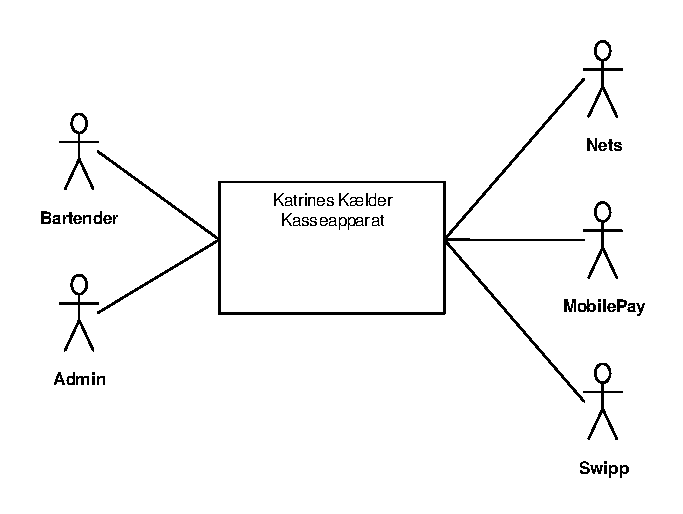
\includegraphics[width=0.8\textwidth]{Kravspecifikation/Actor/Actor.pdf}
	\caption{Aktør-kontekst diagram}
	\label{fig:actordiagram}
\end{figure}

\newpage
\subsection{Bartender}
\begin{usecase}
\addtitle{Aktørnavn}{Bartender} 
\addfield{Type:}{Primær}
\addfield{Beskrivelse:}{}
\end{usecase}

\subsection{Admin}
\begin{usecase}
\addtitle{Aktørnavn}{Admin} 
\addfield{Type:}{Primær}
\addfield{Beskrivelse:}{}
\end{usecase}

\subsection{Nets}
\begin{usecase}
\addtitle{Aktørnavn}{Nets} 
\addfield{Type:}{Sekundær}
\addfield{Beskrivelse:}{}
\end{usecase}

\subsection{MobilePay}
\begin{usecase}
\addtitle{Aktørnavn}{MobilePay} 
\addfield{Type:}{Sekundær}
\addfield{Beskrivelse:}{}
\end{usecase}

\subsection{Swipp}
\begin{usecase}
\addtitle{Aktørnavn}{Swipp} 
\addfield{Type:}{Sekundær}
\addfield{Beskrivelse:}{}
\end{usecase}